\chapter{Results}
\label{ch:results}

This chapter examines the results achieved through our experimental work.
Starting off we will show the resulting models through pyLDAvis in Section \ref{results:pyldavis}. The topics are evaluated and compared with a coherence score in Section \ref{results:coherence}. The tables show multiple topics with their top terms in Section \ref{results:topics}. The document distribution based on most relevant topic after applying the model on the corpus in Section \ref{results:doc_distribution}. Ending with a silhouette coefficient score for the models in Section \ref{results:silhouette}. The models were generated using the gensim package and the results compare the train, test and held out data where applicable. 



\section{Model results}\label{results:modelresults}
Our results are created and evaluated with multiple aspects in mind. The human interpretation and semantic analysis of the documents have been leading for our models and results. Each section discusses one of these aspects. The experiments are conducted with the gensim package. The models have been created with 2 till 38 topics. The default settings in gensim allowed our models to be trained on our test and train data, further explained in Section \ref{methodology:model_building}. Section \ref{results:wordcloud} - \ref{results:coherence} used only the train and test data, the remaining sections compare the held out data.

\FloatBarrier
\section{Wordcloud}\label{results:wordcloud}
We represented our terms in a wordcloud, Fig \ref{fig:worldcloud}, which as the name implies simply shows the terms in the topics created by our models in a cloud. Nothing special so far to behold, but a quick glance on the words show words which are very domain specific as such we cannot easily interpret the meaning behind the words or their relation.

 \begin{figure}[h]
    \centering
    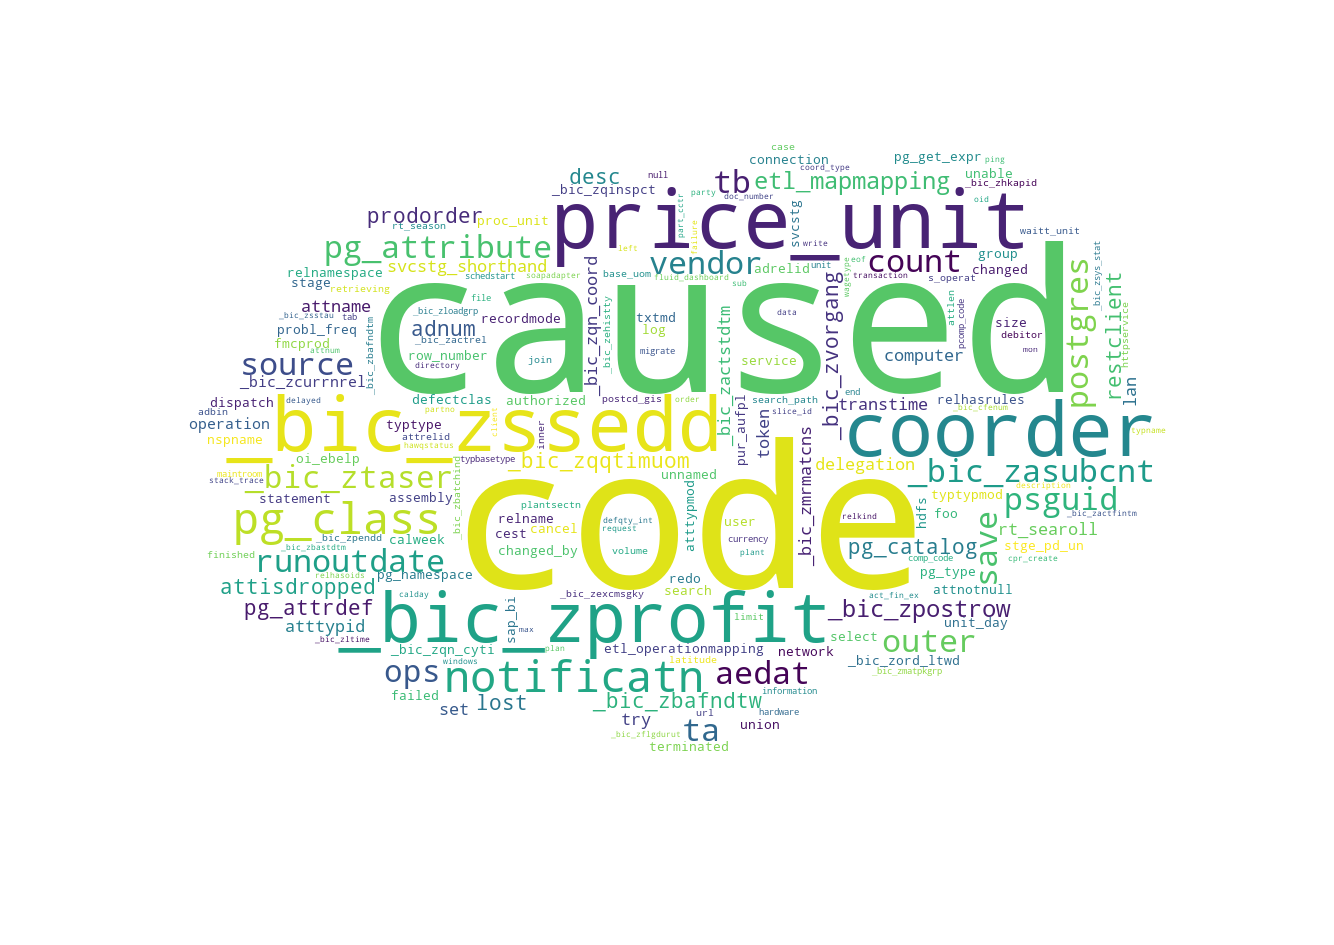
\includegraphics[width=15cm, height=8cm]{figures/wc.png}
    \caption{A wordcloud containing terms found in clusters}
    \label{fig:worldcloud}
\end{figure}

\FloatBarrier

\section{Topic overview}\label{results:topics}
First we examine the latent topics our models have generated. We showcase the topic count 2, 5 and 10. We will use these as a reference for further topic exploration. The remaining topics can be found in the Appendix A \ref{appendices:modelgeneratedtopics}. Our topics are shown in Table \ref{tab:2topicsmodel}, \ref{tab:5topicsmodel}, \ref{tab:10topicsmodel}. The topics should provide a clear view of the type of errors in our dataset.

\begin{table}[h]
\centering
\begin{tabular}{|l|l|l|l|l|l|}
 \hline
 Topic & Terms & & & & \\
 \hline
 \hline
 0 & user & information & retrieving & ta & select\\ 
 \hline 
 1 & failed & code & request & restclient & ping\\ 
 \hline 
\end{tabular}
\caption{Topic 1..2 with top 5 terms}
\label{tab:2topicsmodel}
\end{table}

Examining Table \ref{tab:2topicsmodel}, we cannot simply deduce what these two topics are about. We can at best say that the second topic is probably an error topic based on the simple word failed. The topic count is fairly low and earlier exploration expects us to have more latent topics in the dataset. The extracted topics are probably the most common occurring terms. This is actually true if we compare these topics with Fig \ref{fig:Termfreq}.


\begin{table}[h]
\centering
\begin{tabular}{|l|l|l|l|l|l|}
 \hline
 Topic & Terms & & & & \\
 \hline
 \hline
 0 & ta & select & f & group & plan\\ 
 \hline 
 1 & fluid\_dashboard & text & tblasset\_ser & tbljob\_sow & group\\ 
 \hline 
 2 & v & r & order & null & tb\\ 
 \hline 
 3 & failed & code & request & source & restclient\\ 
 \hline 
 4 & user & information & retrieving & log & party\\ 
 \hline 
\end{tabular}
\caption{Topic 1..5 with top 5 terms}
\label{tab:5topicsmodel}
\end{table}

We continue on to our next table, Table \ref{tab:5topicsmodel}. We see similar words in this table as Table \ref{tab:2topicsmodel}, topic 3 and 4 have the same terms as topic 0 and 1 in the first table. It is probable that these terms are common occurrences throughout our corpus. Once again looking at our Fig \ref{fig:Termfreq}, we recognise more common terms. Although the count of topics has increased our ability to deduce the topics has not been increased.
 
\begin{table}[h]
\centering
\begin{tabular}{|l|l|l|l|l|l|}
 \hline
 Topic & Terms & & & & \\
 \hline
 \hline
 0 & request & migrate & restclient & url & ping\\ 
 \hline 
 1 & fluid\_dashboard & text & tblasset\_ser & tbljob\_sow & coord\_type\\ 
 \hline 
 2 & ordcateg & cancel & token & postgres & \_bic\_zpmrsord\\ 
 \hline 
 3 & orderitem & redo & record & unit\_day & length\\ 
 \hline 
 4 & f & foo & count & ta & v\\ 
 \hline 
 5 & ops & hawqstatus & down\_indic & set & \_bic\_zlongit\\ 
 \hline 
 6 & request & ping & migrate & url & http\\ 
 \hline 
 7 & failed & material & recordmode & notificatn & group\\ 
 \hline 
 8 & ta & select & group & plan & dispatch\\ 
 \hline 
 9 & user & information & retrieving & tblasset\_ser & tbljob\_sow\\ 
 \hline 
\end{tabular}
\caption{Topic 1..10 with top 5 terms}
\label{tab:10topicsmodel}
\end{table}

The final table is Table \ref{tab:10topicsmodel}. Once again the topics are hard to read, although some topics have become more clear. Topic 2 and 3 are probably about database changes to orders. The terms "failed" and "user" are once again shown, except "failed" is now grouped with a very different set of terms. Some terms appear more times, e.g. "ta" and "tbljob\_sow", "url". It shows us that more latent topics are hidden within our dataset, which the low count of 2 and 5 topics cannot show. However due to the ambiguity of the terms we cannot tell if we need more topics to generalise or reduce the amount to make topics more specific.

The remaining topics shown. Trying to infer topics through the top terms has so far left a undesirable result. Servers logs which are created for domain specific programs and systems make it harder to interpret a coherent and distinctive topic. Noticeably in higher topic counts the amount of similar top terms, e.g. term 'ta' in the model with 11 topics appears 3 times as top term in 3 separate topics. This might simply be a popular word for multiple documents or the model is not sufficient. Lower topic counts have topics which are clearly not representing the smaller and important infrequent occurring server log messages.

The results leave us with the desire to better interpret the topics and gave us a clear view that interpreting is not an easy task.

\FloatBarrier
\section{Comparison of the inferred topics through pyLDAvis}\label{results:pyldavis}
In this section we will discuss the inferred mapping of pyLDAvis. The visual representation of 5 topics in Fig \ref{fig:pyldavis_5} and of 10 topics in Fig \ref{fig:pyldavis_10} will be used to compare other models. The pyLDAvis mapping includes the distance metric Jensen Shannon and as such computes distance of each topic to each other, as mentioned before at Section \ref{methodology:humanperception}. The package allows closer inspection of topics through term relevance. It does not show the reality of the documents being clustered, only an estimate of the topic size compared to other topics based on the term frequency. The remaining topics can be found at Appendix A \ref{appendices:pyldavis}. 

\begin{figure}[h]
    \centering
    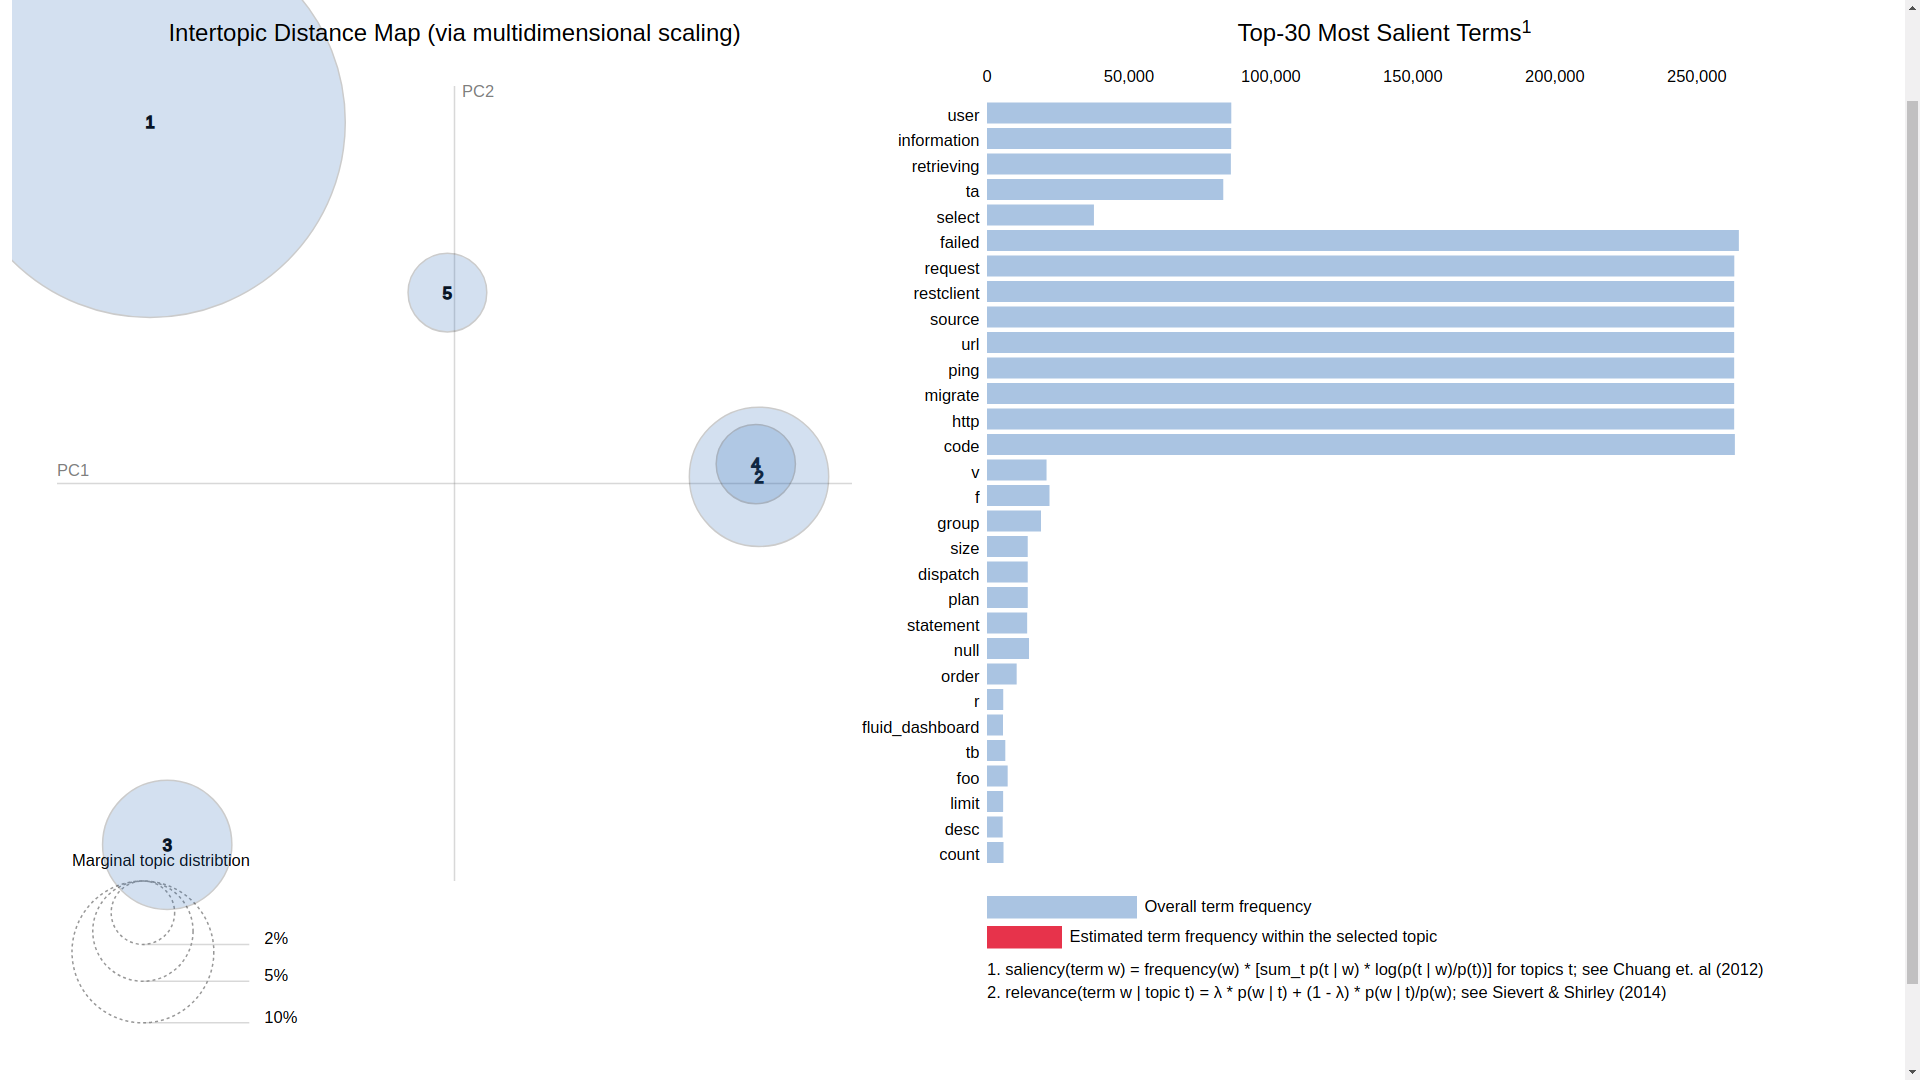
\includegraphics[width=15cm, height=8cm,trim=0 0 100px 0, clip=true]{figures/pyldavis/pyldavis_5.png}
    \caption{pyLDAvis topic visualisation with 5 topics}
    \label{fig:pyldavis_5}
\end{figure}
\FloatBarrier

We first inspect Fig \ref{fig:pyldavis_5}.
Interestingly the figure implies that there is already an overlap of topics with as few as 5 topics. Topics 2 and 4 are overlapping, this could simply be a result of the dimensional reduction applied by pyLDAvis, meaning topics have overlapping terms. The remaining topics have a clear distance from each other. Although topic 1 is very large, it is expected though because the dataset contained a lot of similar terms.

\begin{figure}[h]
    \centering
    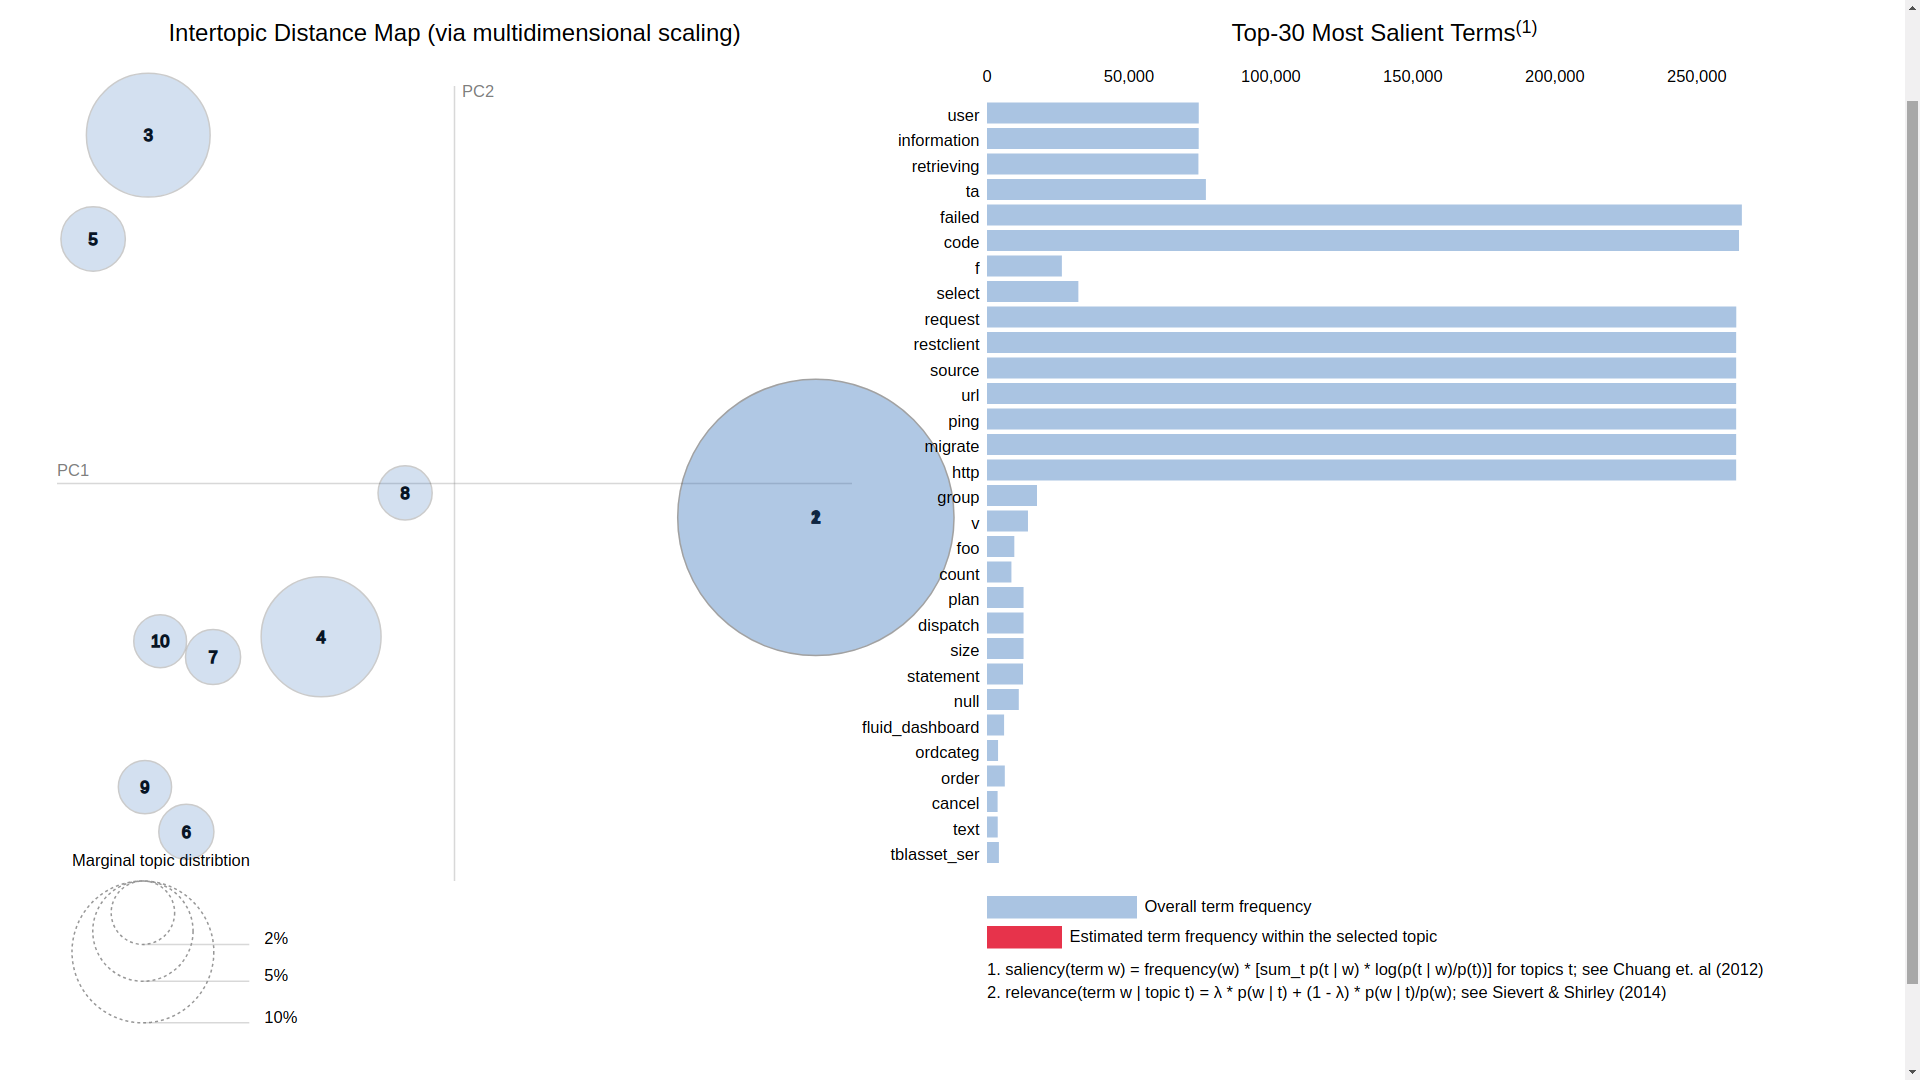
\includegraphics[width=15cm, height=8cm,trim=0 0 100px 0, clip=true]{figures/pyldavis/pyldavis_10.png}
    \caption{pyLDAvis topic visualisation with 10 topics}
    \label{fig:pyldavis_10}
\end{figure}

In Fig \ref{fig:pyldavis_10} we jump to 10 topics. Closer inspection of the pyLDAvis shows overlap in topic 1 and 2. The remaining topics are reasonably well distinguished and show no overlap. 

Further examining the remaining figures we like to state the following:
\begin{enumerate}
  \item The remaining figures show no clear preference of topic count
  \item The majority of figures appear to have overlapping topics
\end{enumerate}
The first statement is probably because pyLDAvis is created to help show a global topic distinctiveness but also help the user interpret the topics relevant term. This means it is not necessarily built for different topic count comparison. The second statement is once again due to the nature of LDA which has overlapping terms in different topics, like the topics in 1 and 2 in the 10 topics model.

\FloatBarrier
\section{Coherence}\label{results:coherence}
The next results show a topic coherence score in correlation to topic count. In comparison to earlier results, we use a calculated score rather than our own judgement. The coherence model is based on the coherence measure Cv, which measure human interpretability. Hopefully the results make show a topic count with a clear  Our Fig \ref{fig:coherence} shows the average value each model scored. 

 \begin{figure}[h]
    \centering
    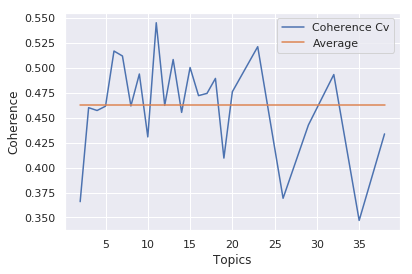
\includegraphics[width=15cm, height=8cm]{figures/coherence_values_topics.png}
    \caption{Coherence values based on the measure Cv}
    \label{fig:coherence}
\end{figure}

The results in the figure are interesting. As we already discussed in earlier sections, we did not find a clear topic count to be better based on our visual interpretation. The figure shows that topic count 11 has the highest score with 23 being the second highest, in contrast topic count 35 has the lowest. When we look at topic count 11 in Table \ref{tab:11topicsmodel}, we see multiple similar top terms. The topic count 11 also shows a lot of overlapping topics in pyLDAvis. The figure also shows a clear fluctuating score from low to high topic count. The average score is $~0.46$ and 13 of the total 25 topics are above average. Solely based on this figure we could say that 11 has to be the best topic count, however our previous evaluation measures do not clearly agree with this so far.

\FloatBarrier
\section{Document distribution based on hard clustering}\label{results:doc_distribution}
This is the first section where we compare held out data to the train and test data. The models transformed the data into document and topic distributions. Our Fig \ref{fig:doc_distr_1-11corpus} and Fig \ref{fig:doc_distr_1-11held_out} represent the count of documents labelled with their highest probable topic count. The figures show to topic count 2 till 11. The remaining document distributions are found in append A \ref{appendices:documentdistribution}.

\begin{figure}[h]
    \centering
    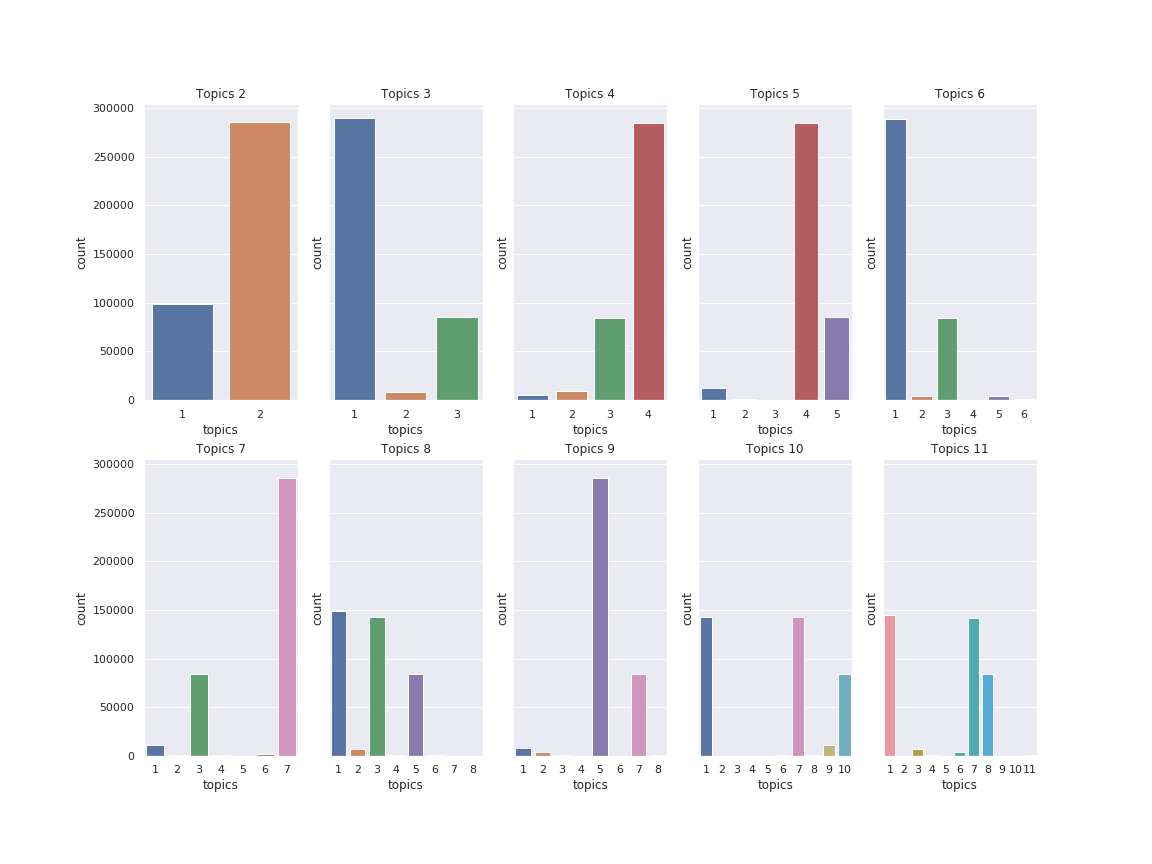
\includegraphics[width=16cm, height=12cm]{figures/doc_distr/doc_distribution_1-11_corpus.png}
    \caption{Document distribution on the train test data}
    \label{fig:doc_distr_1-11corpus}
\end{figure}
\FloatBarrier

The results that are shown in Fig \ref{fig:doc_distr_1-11corpus} are actually very agreeable with what we have seen so far. The distributions based on the topics in pyLDAvis as well the term frequency match up. What we could not see clearly before was how the document would be distributed based on clustering in higher topic counts. Most documents are highly related to at least 2 topics, otherwise 3 topics. The remaining topics are either empty or so small in comparison that our figure cannot show them clearly. If we take a look at the results in the appendix A \ref{appendices:documentdistribution}, which contain our higher topic counts we can see a high variety of distributions. One thing is clear that the increase of topic counts, increases the smoothness of the distribution of documents. A few exceptions have either a singular or duo of topics which contain noticeably more documents. Our results show that increasing the topic count while the corpus does not contain so much latent topic decreases the distinctiveness quality of each topic and as such flattens the distribution of documents.

\begin{figure}[h]
    \centering
    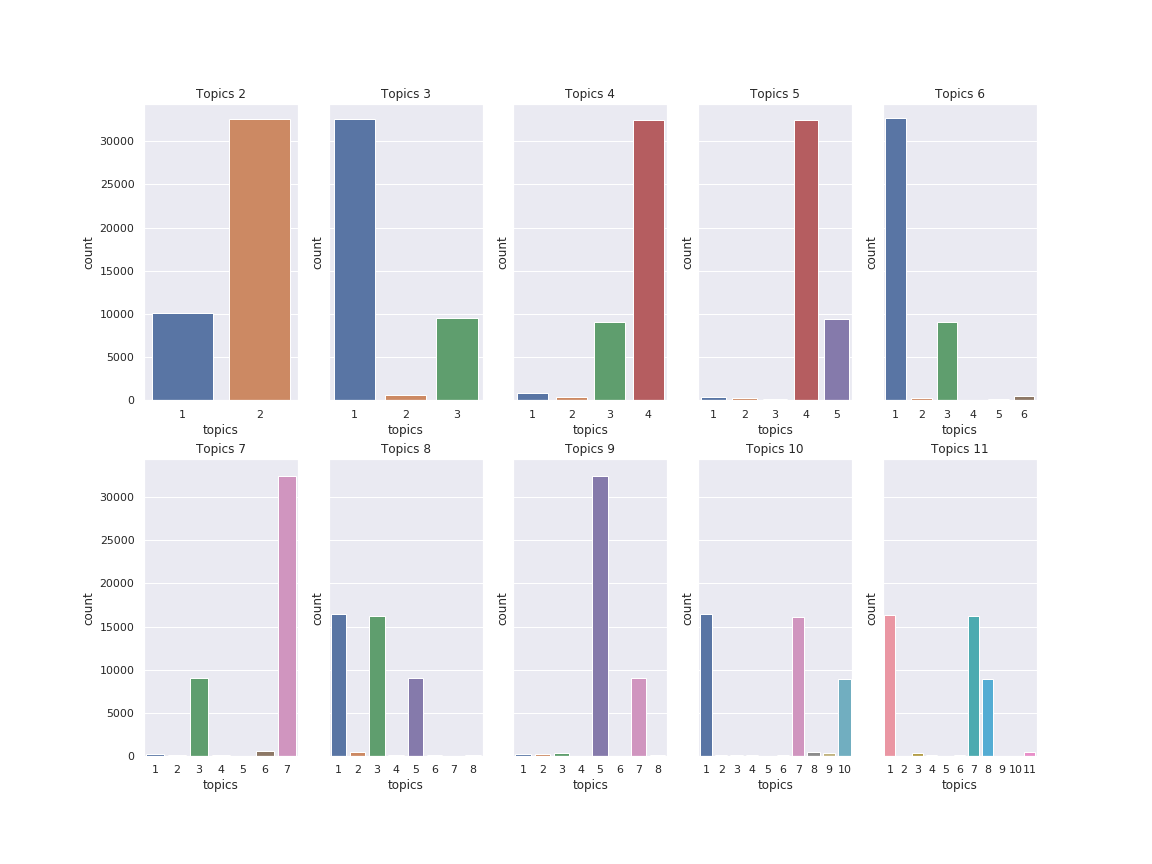
\includegraphics[width=16cm, height=12cm]{figures/doc_distr/doc_distribution_1-11.png}
    \caption{Documents distribution on the held out data}
    \label{fig:doc_distr_1-11held_out}
\end{figure}
\FloatBarrier

The same can be repeated for Fig \ref{fig:doc_distr_1-11held_out}. Although the held out data is created after shuffling the data and then splitting it, the distribution of documents in each model is remarkably similar. The held out dataset appears to be very similar to the train and test data based on the clustering. Which also brings us to the same deduction as before. As we expected, the results in the appendix appear similar. 

In this first comparison between held out and our trained models, we see that results are quite similar. The results have shown that increasing the topic count leads to more evenly distributed documents. The model shows the same output on held out and the train and test data. This is great news as such, this model might be able to indicate errors similar to the topic count of choice. 
\FloatBarrier

\section{Silhouette values}\label{results:silhouette}
The final evaluation metric is the silhouette, which will use the cosine metric. The complexity and memory requirements of silhouette leaves us with a sampled set to be evaluated. Our held out and train and test data are sampled on 10000 documents and hard clustered based on their highest probable topic. It appears to be impossible to calculate the silhouette after 12 topics. The mathematical explanation is that the denominator has a value of zero, as such it can not calculate the silhouette of a sample. This means that topics have become so small and overlapping that the average distance for each sample in a cluster and the nearest cluster has become 0. Silhouette gives a clear score that can only be between -1 and +1, the higher the silhouette score the better our models.

\begin{figure}[h]
    \centering
    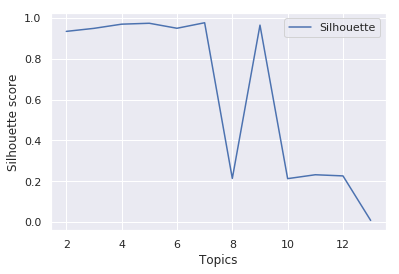
\includegraphics[width=15cm, height=8cm]{figures/silhouette_values_topics_corpus.png}
    \caption{Silhouette values based on the train test data}
    \label{fig:Train test dataset}
\end{figure}
\FloatBarrier

The results shown in our Fig \ref{fig:Train test dataset} show a higher score of silhouette on the lower end, being constantly around 0.9 to 1.0. The only topics that show lower values are topic 8 and all topics after topic count 9. The results do show a preference for lower topic counts, increasing the topic count after 7 topics decreases the silhouette score in general. 

\begin{figure}[h]
    \centering
    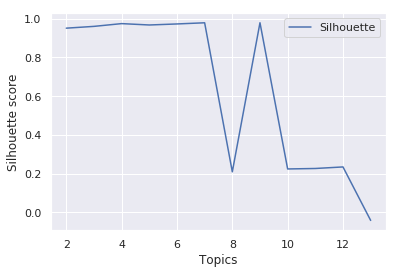
\includegraphics[width=15cm, height=8cm]{figures/silhouette_values_topics_held_out.png}
    \caption{Silhouette score based on the held out data}
    \label{fig:Held out}
\end{figure}

Comparing the Fig \ref{fig:Held out} with the earlier Fig \ref{fig:Train test dataset} shows an expectable similar result. In the previous section we already deduced the held out dataset to be very similar to our train and test dataset. The models show great promise based on the score of the silhouette, although it is noticeable that even the lowest topic count of 2 has a high silhouette score. The silhouette score can be said to evaluate the models based on their created document clusters, which appear to be of great quality. 

\FloatBarrier
\section{Contribution}\label{results:contribution}
In this section we will discuss the specific findings from our research. These findings include the data extraction and exploration of server logs. Applying the online LDA model on the dataset and the general difficulty of evaluating the models. 

The data extraction has been interesting, having access to such a huge amount of data for exploration is a treat for every researcher. In the past research has been performed on extracting server logs for analyses, but not a lot of research is performed with access to a great quantity of data as has been used in this thesis. Furthermore, our data can be said to be unique in the aspect of having typical labels, which identify the type of server logs. 

The identifying process of the dataset has been a main focus. As such we found the LDA machine learning model suitable to provide our dataset with the necessary structure. Topic modelling on server logs for added value has not been done with much success or without much effort in the past. The nature of LDA, makes it hard to evaluate. LDA can be evaluated using metrics which show to have a good performance for extracting latent topics however this can easily contradict human interpretation. The nature of this dataset makes it hard for humans to understand it without domain knowledge, even domain experts might not be enough. However, LDA depends on the readability of its users, entailing us to find the best combination or spot between semantic analysis and human dependability.

The results shown in our Chapter \ref{ch:results}, show interesting results and even contradicting results. The latent topics inferred were evaluated on distinctiveness and coherence. We took a brief look in Section \ref{results:topics} of our topics with their terms and experienced the difficulty hands on of interpreting these topics and choosing the optimal number of topics. Following we use pyLDAvis, which is widely used for topic distinctiveness interpretation and easy interpretation of topics itself. Furthermore, we evaluated the coherence of topics with coherence metric Cv. Finally, we chose to hard cluster the documents in their most probable topics using the silhouette coefficient to see that similar documents are indeed clustered together for certain amount of topics, corresponding with our held out dataset for final confirmation of the quality of our models.

We will discuss the final conclusion drawn from our experiments and answer the general research question in the conclusion next chapter.

\begin{comment}
I dont think I contributed a lot to the research in this area, but I learned a lot right??
\end{comment}
